\documentclass[12pt, a4paper]{article}
\usepackage[utf8]{inputenc}
\usepackage[T2A]{fontenc}
\usepackage[russian]{babel}
\usepackage[oglav,spisok,boldsect,eqwhole,figwhole,hyperref,hyperprint,remarks,greekit]{fn2kursstyle}



\usepackage{subfig}
%\usepackage{amsmath}
%\usepackage{amssymb} 
\usepackage{amsfonts}
\usepackage{mathtools}
\usepackage{enumitem}
\usepackage{pifont}
\usepackage{changepage}
\usepackage{multirow}
\usepackage{supertabular}
\usepackage{multicol}
\usepackage{scalerel}
%\usepackage{txfonts}


\graphicspath{
	{./style/}
	{../wolfram/f_22600_10.08.26/plots/}
	{../wolfram/f_22601_10.08.26/plots/}
	{../wolfram/f_22609_10.08.25/plots/}
	{../wolfram/f_22608_10.08.28/plots/}
	{./illustr/}
}

%\usepackage{multirow}
%\usepackage{supertabular}
%\usepackage{multicol}

\frenchspacing
\sloppy
\counterwithout{equation}{section}
\counterwithout{figure}{section}
\newenvironment{comment}{}{}




% Параметры титульного листа
\title{Поиск потенциала электрического поля в периодической структуре}
\author{А.\,Д.~Егоров}
\supervisor{К.\,Е.~Казаков}
\group{ФН2-62Б}
\date{2023}

% Переопределение команды \vec, чтобы векторы печатались полужирным курсивом
\renewcommand{\vec}[1]{\text{\mathversion{bold}${#1}$}}%{\bi{#1}}

\renewcommand{\phi}{\varphi}
\newcommand\Tau{\scalerel*{\tau}{T}}

\newcommand\thh[1]{\text{\mathversion{bold}${#1}$}}
%Переопределение команды нумерации перечней: точки заменяются на скобки
%\renewcommand{\labelenumi}{\theenumi)}
\renewcommand{\labelenumii}{\arabic{enumi}.\arabic{enumii}}
\renewcommand{\labelenumiii}{\arabic{enumi}.\arabic{enumii}.\arabic{enumiii}}
\renewcommand{\labelenumiv}{\arabic{enumi}.\arabic{enumii}.\arabic{enumiii}.\arabic{enumiv}}


\begin{document}
	
	\maketitle	
	\tableofcontents
	\newpage
	
	\section-{Введение}
		
	
	\section {Постановка задачи}
		
		Найти потенциал электрического поля между двумя бесконечными пластинами, профиль одной из которых плоский, а профиль другой описывается некоторой периодической функцией. Значения потенциала на пластинах заданы и константны.		
		
		
	%\newpage
	\section{Обзор задачи}
	
		
		\subsection{Физическая составляющая задачи}
			\looser{-0.02}{Для постоянного электрического (электростатического) поля уравнения Максвелла имеют вид}
			\begin{equation}
				\mathrm{div} \vec{\mathrm{E}} = 4 \pi \rho,
				\label{div_E}
			\end{equation}
			\begin{equation}
				\mathrm{rot} \vec{\mathrm{E}} = 0,
				\label{rot_E}
			\end{equation}
			где $\rho$ --- объемная плотность внешних зарядов. Электрическое поле $\vec{\mathrm{E}}$ выражается через только скалярный потенциал соотношением
			\begin{equation}
				\vec{\mathrm{E}} = -\mathrm{grad} \varphi,
				\label{E_grad_phi}
			\end{equation}
			подставляя (\refeq{E_grad_phi}) в (\refeq{div_E}), получим уравнение, которому удовлетворяет потенциал постоянного электрического поля:
			\begin{equation}
				\Delta \varphi = - 4 \pi \rho.
				\label{Pois_eq}
			\end{equation}
			Уравнение (\refeq{Pois_eq}) есть уравнение Пуассона. При $\rho = 0$, т.е. при отсутствии внешних сил, потенциал удовлетворяет уравнению Лапласа
			\begin{equation}
				\Delta \phi = 0.
				\label{Laplace_eq}
			\end{equation}
			
		\subsection{Математическая постановка задачи}
			
			Из условия поставленной задачи известно, что внешних сил нет, следовательно, потенциал электростатического поля должен удовлетворять уравнению (\refeq{Laplace_eq}). Через функцию $w(x)$ зададим профиль искривленной пластины, $w(x)$  --- некоторая периодическая функция с периодом $T$, т.е. $w(x) = w(x + T)$. Пусть плоская пластина находится над искривленной на уровне $y_a$. Значение потенциала на пластинах заданы и константны, обозначим значение на верхней (плоской) пластине как $\phi_a$, на нижней (искривленной) --- $\phi_w$. Так как профиль профиль задан периодической функцией, следовательно необходимо использовать условие равенства потенциалов в точках $x$ и $x + T$, т.е. $\phi (x, y) = \phi (x + T, y)$.
			
			Из этих условий составим систему, которую требуется решить: 		
			\begin{equation}
				\begin{cases}
					\Delta \phi (x, y)  = 0, \\
					\phi (x, y_a) = \phi_a, \\
					\phi (x, w(x)) = \phi_w, \\
					\phi (x, y) = \phi (x + T, y),\\
					
				\end{cases}
			\end{equation}
			\begin{figure*}[!h]
				\centering
				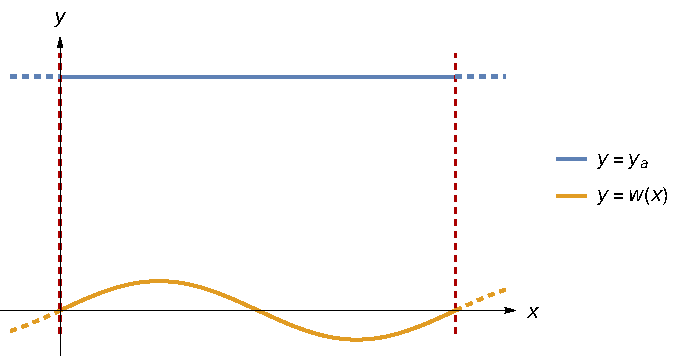
\includegraphics[width=0.65\textwidth]{illustr.pdf}
				\caption{Иллюстрация области, в которой будет решаться задача}
				\label{fig:illustr_1}
			\end{figure*}
	
	
	\section{Решение двумерного уравнения Лапласа}
		
		
		\subsection{Аппроксимация уравнения Лапласа методом конечных элементов}
		
			Рассмотрим уравнение Лапласа в двумерной области $\Omega \subset \mathbb{R}^2$
			\begin{equation*}
				\begin{cases}
					- \Delta u  = 0 \ \  \text{в}\ \  \Omega, \\
					u = g \ \ \text{на}\ \  \Gamma_D,
				\end{cases}			
			\end{equation*}
			где $\Gamma_D$ --- часть границы области, на которой заданы граничные условия первого рода, $\Gamma_D = \partial \Omega,$  $\Gamma_D \ne \emptyset$. 
			
			Опираясь на сведения из источника \cite{Galanin}, представим решение задачи в виде $u = u_0 + u_g$, где функция $u_0$ обращается в ноль на границе $\Gamma_D$б а $u_g$ --- некоторая, произвольная, но наперед заданная функция, значения которой совпадают с $g$ на границе области, $u_g |_{\Gamma_D} = g$.
			
			И переходим к следующей задаче с однородными граничными условиями первого рода на $\Gamma_D$ относительно функции $u_0$:
			\begin{equation*}
			\begin{cases}
				- \Delta u  = \Delta u_g \ \  \text{в}\ \  \Omega, \\
				u_0 = 0 \ \ \text{на}\ \  \Gamma_D.
			\end{cases}			
			\end{equation*}
			
			\looser{0.0}{Запишем слабую постановку задачи для определения $u_0$, способом описанным в разделе \textbf{16.3.1}} источника \cite{Galanin}: необходимо определить $u_o \in V_D$, такое, что 
			\begin{equation*}
				\int_{\Omega} \nabla u_0 \cdot \nabla v \, d\Omega = 
				- \int_{\Omega} \nabla u_g \cdot \nabla v \, d\Omega, \quad v \in V_D,
			\end{equation*}			
			\looser{-0.014}{где пространство $V_D$ состоит из функций, имеющих суммируемые с квадратом первые производные и обращающихся в ноль на части $\Gamma_D$ границы расчетной области:}
			\begin{equation*}
				V_D = \left\{ v \in V: \ v |_{\Gamma_D} = 0 \right\},
			\end{equation*}
			а пространство $V$ состоит из произвольных заданных в $\Omega$ функций, имеющих суммируемые с квадратом первые производные.
			
			Для аппроксимации задачи с помощью МКЭ рассмотрим конечномерное пространство $V_h$, аппроксимирующее пространство $V$ и пространство 
			$V_{D,h} = V_h \cap V_D(\Omega)$, элементы которого приближают элементы пространства $V_D$. 
			
			Пусть функция $u_{g,h} \in V_h $ представляет собой аппроксимацию функции $u_g$, задающей граничное условие первого рода. В качестве функции $u_{g,h}$. 
			
			Тогда конечномерная задача примет вид: 
			%определить $u_{0,h} \in V_{D,h}$, такую, что
			
			\begin{equation*}
				\int_{\Omega} \nabla u_{0,h} \cdot \nabla v_{h} \, d\Omega = 
				- \int_{\Omega} \nabla u_{g,h} \cdot \nabla v_{h} \, d\Omega, \quad v_{h} \in V_D,
			\end{equation*}
			
			Пусть $\phi_i$, \ i = $\overline{1, N},$ --- базис в пространстве $V_h$, причем часть функций $\phi_i$ с номерами $i \in I$ образуют базис в пространстве $V_{D,h}$, т.е. обращаются в ноль на границе $\Gamma_D$. Количество таких индексов будем считать равным $M = |I| < N,\ |I| > 1$.
			
			Тогда последнее уравнение будет эквивалентно
			\begin{equation*}
				\int_{\Omega} \nabla u_{0,h} \cdot \nabla \phi_{i} \, d\Omega = 
				- \int_{\Omega} \nabla u_{g,h} \cdot \nabla \phi_{i} \, d\Omega, \quad i \in I.
			\end{equation*}
			
			Представляя неизвестное решение в виде линейной комбинации базисных функций:
			\begin{equation*}
				u_{0,h} = \sum_{i \in I} u_{0,h,i} \phi_i, \quad 
				u_{g,h} = \sum_{i = 1}^{N} u_{g,h,i} \phi_i, 
			\end{equation*}
			\looser{-0.0}{окончательно получим СЛАУ для определения неизвестных коэффициентов 
			$U_h = \left\{ u_{0, h, i}\right\}$:}
			\begin{equation*}
				A u_{0,h} = b,
			\end{equation*}
			где $A = A_{M \times M}$ --- матрица жесткости, $b = b_{M \times 1}$,
			\begin{equation}
				A_{ij} = \int_{\Omega} \nabla \phi_i \cdot \nabla \phi_j \, d\Omega,
				\quad i, j\in I,
				\label{A_stiff_first}				
			\end{equation}
			\begin{equation}
				b_i = - \sum_{j=1}^{N} u_{g,h, j} \int_{\Omega} \nabla \phi_i  \cdot \nabla \phi_j \, d\Omega, \quad i \in I.
				\label{b_stiff_first}
			\end{equation}
			
			
		\subsection{Метод конечных элементов на треугольной сетке}
			
			\subsubsection{Триангуляция области}
			
				\looser{-0.012}{Зададим в нашей области $\Omega$ правильную триангуляцию $\Tau$, т.~е. такое разбиение области $\Omega$ на треугольные ячейки, что любые два треугольника имеют либо общее ребро, либо общую вершину, либо пустое пересечение.} Таким образом, 
				\begin{equation*}
					\Omega = \underset{T \in \Tau}{\bigcup}T 
				\end{equation*}
				
				Каждый треугольник $T$ при этом задается набором трех своих узлов $P_k$ с координатами $P_k = (x_k, y_k)$. Будем считать, что узлы треугольника обходятся в положительном направлении (против хода часовой стрелки).
				
				Рассмотрим простейший случай: выберем базисные функции $\phi_k$ такие, что $\phi_k$ --- кусочно-линейная функция, принимающая значение единица в узле $P_k$ и ноль во всех остальных узлах. В пределах одного треугольника она продолжена линейно.
				
				В силу аддитивности интеграла относительно области интегрирования  формулы (\refeq{A_stiff_first}) и (\refeq{b_stiff_first}) могут быть записаны в виде			
				\begin{equation}
					A_{ij} = \sum_{T \in \Tau}\int_{T} \nabla \phi_i \cdot \nabla \phi_j \, d\Omega,
					\quad i, j\in I,
					\label{A_stiff_second}				
				\end{equation}
				\begin{equation}
					b_i = - \sum_{j=1}^{N} u_{g,h, j} \sum_{T \in \Tau} \int_{T} \nabla \phi_i  \cdot \nabla \phi_j \, d\Omega, \quad i \in I.
					\label{b_stiff_second}
				\end{equation}
				
				Таким образом, задача вычисления интегралов для коэффициентов матрицы жесткости задачи и ее правой части сводится к задаче вычисления тех же интегралов по отдельным треугольникам.
				
				
				Рассмотрим один из треугольников $T$ триангуляции $\Tau$. Будем считать, что его вершины имеют координаты  $P_i = (x_i, y_i), \ i=\overline{1,3}$. Пусть $\phi_i, \ i=\overline{1,3}$, --- базисные функции соответствующие этим вершинам и данному треугольнику. Таким образом 
				\begin{equation*}
					\phi_i(x_j, y_j) = \delta_{ij}, \ i,k = 1,2,3.
				\end{equation*}
				Функции $\phi_i$ являются линейными в пределах $T$ и имеют следующий вид
				\begin{equation}
					\phi_i(x,y) = 
					\dfrac{
						\det{
							\begin{pmatrix}
								1 & x & y \\
								1 & x_{i+1} & y_{i+1} \\
								1 & x_{i+2} & y_{i+2} \\							
							 \end{pmatrix}
						 }
					}{
					\det{
						\begin{pmatrix}
							1 & x_{i} & y_{i} \\
							1 & x_{i+1} & y_{i+1} \\
							1 & x_{i+2} & y_{i+2} \\							
						\end{pmatrix}
						}
					}, \quad i = 1,2,3,
					\label{basis_fun_phi}
				\end{equation}
				где для удобства обозначения считается, что $P_4 = P_1, \ x_4 = x_1, \ y_4 = y_1, $ аналогично индекс 5 идентичен индексу 2.
				
				Из формулы (\refeq{basis_fun_phi}) получаем следующие соотношения:
				\begin{equation*}
					\nabla \phi_{i}(x,y) = \dfrac{1}{2 |T|} 
					\begin{pmatrix}
						y_{i+1} - y_{i+2} \\
						y_{i+2} - y_{i+1} \\
					\end{pmatrix},
				\end{equation*}
				где $|T|$ --- площадь треугольника $T$, такая, что
				\begin{equation*}
					|T| = \dfrac{1}{2} 
					det{
						\begin{pmatrix}
							x_2 - x_1 & x_3 - x_1 \\
							y_2 - y_1 & y_3 - y_1 \\
						\end{pmatrix}				
					}.
				\end{equation*}
				
				В результату получаем следующее выражение для матрицы жесткости конечного элемента $T$:
				\begin{eqnarray}
					A_{T,ij} = \int_{T} \nabla \phi_i \cdot \nabla \phi_j \, d\Omega
					= \dfrac{|T|}{(2|T|)^2} 
					\begin{pmatrix}
						y_{i+1} - y_{i+2}\\
						x_{i+2} - x_{i+1}\\
					\end{pmatrix}^T
					\begin{pmatrix}
						y_{j+1} - y_{j+2}\\
						x_{j+2} - x_{j+1}\\
					\end{pmatrix},
					\quad i,j=1,2,3.
					\label{A_stiff_in_T}
				\end{eqnarray}
				
			\subsubsection{Сборка глобальной матрицы жесткости}
				
				В предыдущем пункте было рассмотрено, как составляется матрица жесткости для одного элемента $T$ триангуляции $\Tau$. Основываясь на формулах (\refeq{A_stiff_second}, \refeq{b_stiff_second}, \refeq{A_stiff_in_T})  имеем: 
				\vspace*{-6mm}
				\begin{table}[!h]
					\begin{center}
						\begin{tabular}{|c|c|}
							\hline
							\multicolumn{2}{|c|}{Для каждого элемента $T$ триангуляции $\Tau$} \\
							\hline
							$A_T$ & симметричная матрица размером $3 \times 3$,\\
							\hline
							$\vec{b}_T$ & вектор правой части, состоящий из 3, компонент\\
							\hline
							$\vec{u}_T$ & вектор неизвестных, состоящий из 3 компонент.\\
							\hline
						\end{tabular}
					\end{center}
				\end{table}
				\vspace*{-6mm}
								
				\noindent
				Для решения задачи необходимо составить полную систему $A\vec u = \vec b$, где $A$ --- матрица жесткости размером $N \times N$, $\vec b$ --- вектор правой части длины $N$, $\vec u$ --- вектор неизвестных длины $N$, $N$ --- количество узлов триангуляции $\Tau$, для этого нужно собрать все локальные матрицы жесткости $A_T$, т.~е. учесть вклад каждого конечного элемента.
				
				Проиллюстрируем эту процедуру на примере. У нас есть треугольник $T$, составленный из узлов $P_1 = (x_1, y_1), \ P_3 = (x_3, y_3), \ P_5 = (x_5, y_5)$ (номера узлов взяты из глобальной нумерации), для него были получены следующая матрица жесткости $A_T$ и вектор правой части $b_T$
				\begin{equation*}
					A_T = \begin{pmatrix}
						\phantom{-}1.3 & -0.5 & \phantom{-}7 \\
						-0.5 & -0.45 & \phantom{-}0.3 \\
						\phantom{-}7 & \phantom{-}0.3 & \phantom{-}2.1 \\
					\end{pmatrix},
					\quad
					\vec b_T = \begin{pmatrix}
						2 \\
						2.1 \\
						1 \\
					\end{pmatrix}.
				\end{equation*}
				Допустим, что полная система состоит из 7 узлов. Тогда мы расширяем матрицу $A_T$ до размера $7 \times 7$, добавляя нулевые строки и столбцы на место отсутствующих узлов, аналогично для вектора 
				$\vec b_T$. Таким образом получаем следующие матрицу и вектор правой части
				\begin{equation*}
					\widehat A_T = 
					\begin{pmatrix}
						\phantom{-}1.3 & 0 & -0.5         & 0 & \phantom{-}7   & 0 & 0\\
						  \phantom{-}0 & 0 & \phantom{-}0 & 0 & \phantom{-}0   & 0 & 0\\
						          -0.5 & 0 & -0.45        & 0 & \phantom{-}0.3 & 0 & 0\\
						  \phantom{-}0 & 0 & \phantom{-}0 & 0 & \phantom{-}0   & 0 & 0\\
					   	  \phantom{-}7 & 0 &\phantom{-}0.3& 0 & \phantom{-}2.1 & 0 & 0\\
						  \phantom{-}0 & 0 & \phantom{-}0 & 0 & \phantom{-}0   & 0 & 0\\
						  \phantom{-}0 & 0 & \phantom{-}0 & 0 & \phantom{-}0   & 0 & 0\\
					\end{pmatrix},
					\quad
					\widehat{\vec b}_T = \begin{pmatrix}
						2 \\
						0 \\
						2.1 \\
						0 \\
						1 \\
						0 \\
						0 \\
					\end{pmatrix}.
				\end{equation*}
				
				Тогда для полной системы матрица $A$ и вектор правой правой части $b$ имеют следующий вид
				\begin{equation}
					A = \sum_{T \in \Tau} \widehat{A}_T, \quad 
					\vec b = \sum_{T \in \Tau} \widehat{\vec b}_T
				\end{equation}
				
				
			
			
			
			
		
			
		
			

	\newpage
	\section{Программная реализация алгоритма}
		
		Построение сеток --- Wolfram Mathematica, алгоритм метода конечных элементов реализован на языке C++
	
	\section-{Заключение}
	
	
	\newpage
	
	\begin{thebibliography}{4}
		
		\bibitem{Galanin} \looser{0.02}{Методы численного анализа математических моделей\,/\,М.\,П.~Галанин,} Е.\,Б.~Савенков. -- 2-е изд., испр. -- Москва : Издательство МГТУ им. Н.\,Э.~Баумана, 2018. -- 591 [1] с.: ил.
		
		
		
		
		
		
		
		
		
	\end{thebibliography}
	

\end{document}